\documentclass[a4paper]{article}

\usepackage[utf8]{inputenc}
\usepackage[spanish,activeacute]{babel}
\usepackage{a4wide}
\usepackage{amsmath}
\usepackage{amsthm}
\usepackage{amsfonts}
\usepackage{graphicx}
\usepackage{tikz}
\usepackage{tkz-graph}
\usepackage{todonotes}
%\usepackage[lined, ruled, linesnumbered]{algorithm2e}
\usepackage[lined, ruled, linesnumbered]{algorithm2e}
\usepackage{caption}	% Para agregar captions de table a entornos tabular
\usepackage{float}
\usepackage{url}
\restylefloat{table}


\title{Trazado de rayos vectorizado}

\date{\today}

\makeindex
\begin{document}

\hfill 
\includegraphics[scale=0.5]{logo1.jpg}~\\[0.25cm]

\begin{center}
	\textbf{\Large Trazado de rayos vectorizado}\\[1cm]
	{\large Martín Mongi Badía\\[0.15cm]}
	Universidad de Buenos Aires\\[0.15cm]
	\texttt{martinmongi@gmail.com}\\[1cm]
\end{center}

\pagenumbering{arabic}
\begin{abstract}
En este trabajo presentamos un algoritmo de trazado de rayos elemental con dos implementaciones: una compilada desde el lenguaje C con GNU Compiler Collection y otra usando las extensiones SIMD de la arquitectura de los procesadores Intel. El objetivo es demostrar la mejora de performance conseguida con la segunda implementación.
\end{abstract}
\hrulefill
\tableofcontents

\clearpage
\section{Introducción}

El trazado de rayos (o \emph{ray-tracing}, como es conocido en inglés) es una técnica usada para la generación de imágenes simuladas que representan objetos posicionados en un espacio tridimensional. Este algoritmo simula el paso de un rayo de luz a través de los pixeles en la imagen a generar, entonces calculando el color que tendría ese píxel si fuera visto a través de una cámara convencional. Este algoritmo tiene alto grado de realismo, si bien es a expensas de un costo computacional alto, lo que no lo hace conveniente para procesos que requieran una respuesta en tiempo real, tales como videojuegos, simuladores, etc. En cambio, este tipo de algoritmos es muy usado en otras aplicaciones donde el tiempo de respuesta no es un inconveniente, tales como la animación de peliculas (algunos ejemplos son \emph{Toy Story} o \emph{Finding Nemo} de Pixar Inc.), o la generación de representaciones realistas de objetos o edificios a construir a partir de planos digitales.
En nuestro algoritmo, implementamos dos primitivas elementales: la esfera o el triángulo. A través de estas, se pueden aproximar prácticamente cualquier objeto que se quiera representar, sin la necesidad de crear una subrutina para cada una de ellos. En la figura 1 se pueden apreciar representaciones de una esfera y un tetraedro generadas por el algoritmo de trazado de rayos. La primera está generada a partir de su primitiva, y el segundo está generado a partir de 4 triángulos, uno por cada cara.\\

\begin{figure}[H]
	\begin{center}
		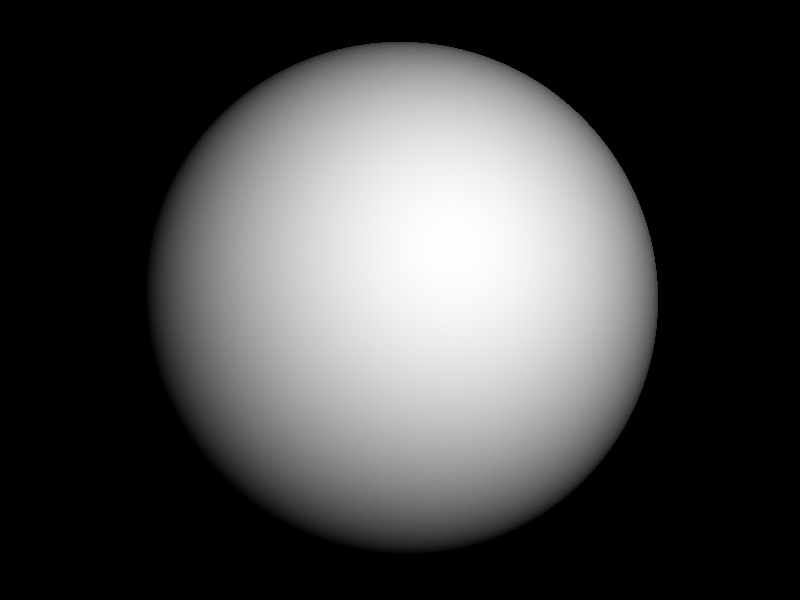
\includegraphics[scale=0.2]{sphere1.jpg}
		\hspace{1.5cm}
		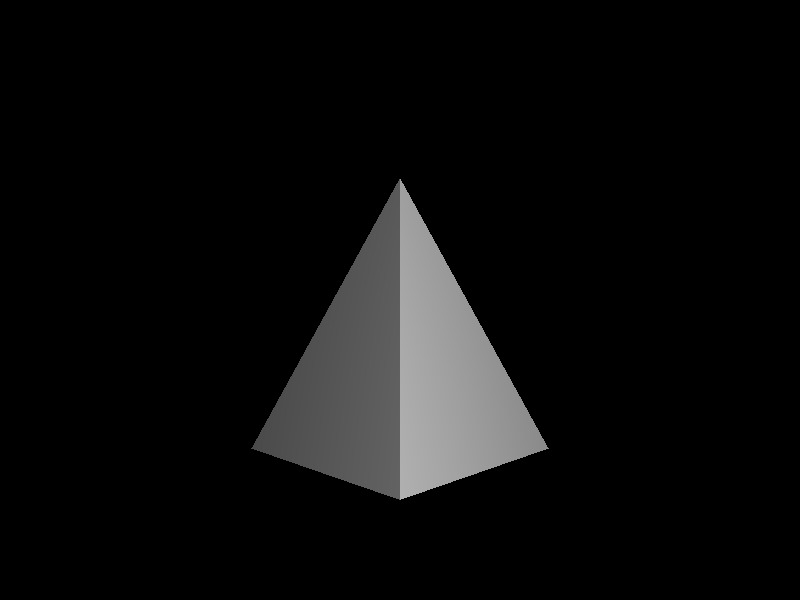
\includegraphics[scale=0.2]{tetrahedron1.jpg}
	\end{center}		
	\caption{Esfera y tetraedro generados por el algoritmo de trazado de rayos}
	\label{fig1}
\end{figure}

Vamos a dividir el trabajo en cuatro partes. En la primera, proveeremos una explicación de los temas de matemática y física que aplicamos para la construcción del algoritmo. En la segunda parte,  explicaremos el algoritmo propiamente dicho, con su correspondiente cálculo de complejidad. En la tercera parte, explicaremos como se llevo a cabo la vectorización de dicho algoritmo, explicando las optimizaciones realizadas. Finalmente, experimentaremos con algunos casos de prueba para medir las mejoras en la práctica que nos da la vectorización y realizaremos el análisis pertinente.
\clearpage
\section{Elementos de matemática y física}

\subsection{Rayo}

El primer elemento que vamos a modelar va a ser el rayo. Para esto, vamos a asumir que la luz viaja en línea recta, por lo cual, podemos modelarlo como una recta, definiendo a $r_0 \in \mathbb{R}^3$ como su punto de origen y $r_d \in \mathbb{R}^3$ como su dirección Entonces, podemos definir a todos los puntos por los que pasa el rayo como:

\begin{equation}
P = \{p:(\exists t \in \mathbb{R}_{\geq 0}: p = r_0 + t r_d)\}
\end{equation}

\subsection{Esfera}

La primer primitiva que desarrollamos es la esfera. Para cada esfera, definimos a $s_c \in \mathbb{R}^3$ como su centro y $s_r \in \mathbb{R}$ como su radio. Entonces, tenemos que todos los puntos de la superficie de la esfera pueden ser definidos como:

\begin{equation}
P = \{p: ||p-s_c||_2 = s_r\}
\end{equation}

\subsubsection{Intersección con el rayo}

El paso siguiente es verificar si un rayo tiene intersección con la esfera. Para esto, vamos a buscar si hay algún punto que cumpla las definiciones de ambos elementos. Combinando las ecuaciones tenemos:

\begin{equation}
||r_0 + t r_d - s_c||_2^2 = s_r^2
\end{equation}
\begin{equation}
(t r_d + r_0 - s_c) . (t r_d + r_0 - s_c) = s_r^2
\end{equation}
\begin{equation}
t^2 (r_d.r_d) + 2t(r_d.(r_0 - s_c)) + (r_0 - s_c). (r_0 - s_c) - s_r^2 = 0
\end{equation}

Vemos claramente que queda una ecuación cuadrática. Resolviendo por $t$ y reemplazando en la ecuación del rayo vemos que hay tres casos posibles:
\begin{itemize}
\item La ecuación tiene dos soluciones. Luego, el rayo tiene dos intersecciones y por lo tanto, no interseca a la esfera tangencialmente.
\item La ecuación tiene una única solución. Por lo tanto, el rayo interseca a la esfera tangencialmente.
\item La ecuación no tiene soluciones. Por lo tanto, el rayo no interseca a la esfera.
\end{itemize}

\subsection{Triángulo}

Luego, tenemos que modelar el triángulo. Para esto, definimos al triángulo por sus vértices $v_1,v_2,v_3 \in \mathbb{R}^3$. Primero, sabemos que todos los puntos en el triángulo están en el plano en el cual el triángulo está incluido. A este plano lo podemos definir por su vector normal \footnote{El vector normal de un plano es un vector que es perpendicular a todos los puntos del plano.} $n$. Como sabemos que sus tres vértices, y por consiguiente sus lados, están incluidos en el plano, podemos calcular a la normal calculando un vector perpendicular a dos de sus lados:

\begin{equation}
n = (v_1 - v_2) \times (v_1 - v_3)
\end{equation}

\subsubsection{Intersección con el rayo}

Luego, tenemos que verificar si el rayo interseca al plano. Entonces, necesitamos los puntos del rayo que sea perpendicular a la normal. Combinando las ecuaciones tenemos:

\begin{equation}
(tr_d + r_0 - v_1) . n = 0
\end{equation}
\begin{equation}
tr_d . n + (r_0 - v_1) . n = 0
\end{equation}
\begin{equation}
t = \dfrac{(v_1 - r_0) . n}{r_d . n}
\end{equation}

Vemos que hay dos casos: $r_d . n = 0$, entonces el rayo es paralelo al plano, por lo tanto, no se intersecan, y $r_d . n \neq 0$, por lo tanto la ecuación tiene una solución y reemplazando en la ecuación del rayo, tenemos la intersección del plano y el rayo.\\
Luego, necesitamos ver que el punto de intersección esté efectivamente dentro del triángulo. Para esto, alcanza con comprobar que para cada par de vértices del triángulo, el otro vértice está del mismo lado que el punto de intersección. Para esto, supongamos que tenemos dos semiplanos divididos por una recta que pasa por los puntos $a$ y $b$, y queremos ver si los puntos $p_1$ y $p_2$ están en el mismo semiplano. Esto pasa sí y solo sí se cumple lo siguiente:

\begin{equation}
((b - a) \times (p_1 - a)) . ((b - a) \times (p_2 - a)) \geq 0
\end{equation}

\subsection{Superficie de Lambert}

En física, se dice que una superficie es de Lambert o lambertiana, cuando, al recibir luz, esta es reflejada para todas las direcciones con la misma intensidad. Por lo tanto, la intensidad de la luz apreciada no cambia al cambiar el punto de visa, de la forma que lo haría una superficie reflectiva. Una superficie de Lambert es, entonces, una superfice de reflexión difusa ideal. De esta forma, siendo $L$ el vector de la superficie a la fuente de luz, $N$ la normal de la superficie, $C$ el color de la superficie y $I_L$ la intensidad de la fuente de luz, podemos calcular la intensidad de la luz reflejada de la siguiente forma:

\begin{equation}
I_D = (L.N)CI_L
\end{equation}
\section{Desarrollo del algoritmo}

\subsection{Entrada de datos}

Al inicio del programa, este recibe datos a través de un archivo de entrada tales como: nombre y tamaño de imagen de destino, distancia focal de la cámara simulada, cantidad de luces, cantidad de esferas y cantidad de triángulos. Luego, lee las propiedades de cada objeto: intensidad, color y posición para las luces, color, posición y radio para las esferas, y color y posición de los vértices para los triángulos.

\subsection{Trazado de rayos}

Luego, el programa procede a calcular los rayos. Suponiendo que la imagen de destino tiene que ser de $n$ píxeles de alto por $m$ píxeles de ancho, armamos una grilla de ese tamaño, la cual colocamos a la distancia focal de la camara que el programa recibió. Para simplicidad del código, para todos los rayos trazados desde la cámara, tomaremos $r_o = \vec{0}$. Entonces, tomamos los puntos de la grilla como las direcciones de los diferentes rayos que trazaremos.\\
Ahora, necesitamos saber si el rayo se interseca con algún objeto como previamente vimos y, en ese caso, saber cual es el objeto más cercano con el cual se interseca, ya que es el que se vería desde la vista de la cámara. Luego de esto, procedemos a calcular el color del píxel. Para simplicidad del código, suponemos que todas las superficies son lambertianas. Cómo la luz es aditiva, calculamos la luz proveniente de cada una de las fuentes de luz con la fórmula previamente vista. El algoritmo sigue el siguiente pseudocódigo:


\begin{algorithm}
\DontPrintSemicolon

\SetKwInOut{input}{Input}
\SetKwInOut{output}{Output}
\SetKwInOut{signature}{Signatura}

\input{	$\mathbf{i_w}$ ancho de la imagen\\
		$\mathbf{i_h}$ alto de la imagen\\
		$\mathbf{fd}$ distancia focal de la cámara simulada\\
		$\mathbf{Lights}$ luces\\
		$\mathbf{Spheres}$ esferas\\
		$\mathbf{Triangles}$ triángulos\\
		}

\output{$\mathbf{I}$ imagen}

$relation \gets \dfrac{i_w}{i_h}$\;
$w_h \gets \dfrac{35}{\sqrt{relation^2+1}}$\;
$w_w \gets relation \times w_h$\;
$step \gets \dfrac{w_w}{i_w}$\;

\For{$row \gets 1$ \KwTo $i_h$}{
	\For{$col \gets 1$ \KwTo $i_w$}{
		Ray $r$\;
		$r_{d,x} \gets step \times (col + 0.5) - \frac{w_w}{2}$\;
		$r_{d,x} \gets -step \times (col + 0.5) + \frac{w_w}{2}$\;
		$r_{d,z} \gets fd$\;
		$r_o \gets \vec{0}$\;
		$nearest \gets \infty$\;
		\ForAll{$o \in Spheres \cup Triangles$}{
			\If{$intersect(o,r)$}{
				$p \gets intersection(o,r)$\;
				\If{$distance(p,r_o) < nearest$}{
					$nearest \gets distance(p,r_o)$\;
					$I_{row,col} \gets \vec{0}$\;
					\ForAll{$l \in Lights$}{
						$I_{row,col} \gets I_{row,col} + reflection(l, o$)\;
					}	
				}
			}
		}
		
	}
}
\Return $I$
\caption[]{Trazado de rayos}
\end{algorithm}
\clearpage
\subsection{Complejidad temporal}

Como se ve en el algoritmo, el cíclo de las líneas entre 19 y 21 se ejecuta $O(|l|)$ veces. Como el cíclo entre las líneas 13 y 24 se ejecuta $O(|s|+|t|)$ veces, tiene un costo de $O((|s|+|t|) \times |l|)$ Al mismo tiempo, las líneas entre 7 y 24, se ejecutan $O(i_h \times i_w)$ veces, dando una complejidad temporal total de $O((|s|+|t|) \times |l| \times i_w \times i_h)$.
\clearpage
\section{Optimizaciones del modelo SIMD}

El principal objetivo de este trabajo es comprobar las mejoras en performance que se consiguen con la utilización del modelo de instrucciones SIMD (\emph{Single Instruction Multiple Data}) de la arquitectura x86-64 de los procesadores Intel. Este tipo de instrucciones consiguen acelerar las operaciones en los casos en los cuales se necesita aplicar la misma operación a varios datos, consiguiendo efectuar la misma operación en una fracción de los ciclos de procesador necesarios con el modelo convencional. En el caso particual de nuestro algoritmo, hay varias operaciones que pueden ser aceleradas con esta técnica. Por ejemplo, casi cualquier operación con vectores, tales como suma, resta, producto interno, producto cruz, cálculo de norma, etc. puede ser acelerada sin muchos inconvenientes, ya que son operaciones que ejecutan varias veces la misma operación con datos diferentes. También, un ejemplo de esto son las operaciones sobre los píxeles de color. Como los píxeles se guardan en ternas RGB (\emph{red}, \emph{green}, \emph{blue}), las operaciones generalmente son paralelas para cada canal del sistema de color. Como ejemplo, mostramos la cantidad de instrucciones necesarias para hacer algunas de las operaciónes en las dos implementaciones comparadas:\\

{\center
\begin{tabular}[H]{l|r|r}
& Instrucciones compiladas desde C & Instrucciones SIMD\\\hline
Suma de vectores & 35 & 1 \\
Resta de vectores & 35 & 1\\
Producto escalar & 25 & 2\\
Producto interno & 25 & 3\\
Norma 2 de un vector & 26 & 4\\
Producto cruz & 44 & 7\\
\end{tabular}
}\\[1cm]

Además de esta optimización, todas estas operaciones fueron realizadas con macros en la implementación SIMD, lo que reduce el \emph{overhead} por el llamado a funciones, aunque consideramos que el impacto es mínimo en la performance.
\clearpage
\section{Experimentación}

Nuestro equipo de pruebas fue una notebook Lenovo Y40 con procesador Intel\textregistered Core\texttrademark i7-4510U CPU con 2 núcleos físicos y 4 lógicos, corriendo a 2.0 GHz y 16 GB de memoria RAM. Todas las mediciones de tiempo de ejecución fueron tomadas utilizando el TSC (\emph{timestamp counter}), un registro interno del procesador que lleva la cuenta de cuantos ciclos del procesador han pasado desde su último reset. Compilamos la versión en C con el compilador C de GNU Compiler Collection utilizando la opción de optimización \texttt{-O3}. Para cada caso de prueba, corrimos los algoritmos 25 veces y promediamos los tiempos de ejecución, para tener una mejor estimación. En este experimento, compararemos las dos implementaciones del algoritmo. Para esto, utilizamos un conjunto de datos de entrada que consiste en una esfera y una luz que dejamos fijo. Entonces, vamos variando el tamaño de la imagen deseada tomando $i_w \times i_h \in [100000 \dots 2000000]$, para ver si existe la mejora que esperamos con la implementación. En la figura 2 se ven los resultados.\\

\begin{figure}[H]
	\begin{center}
		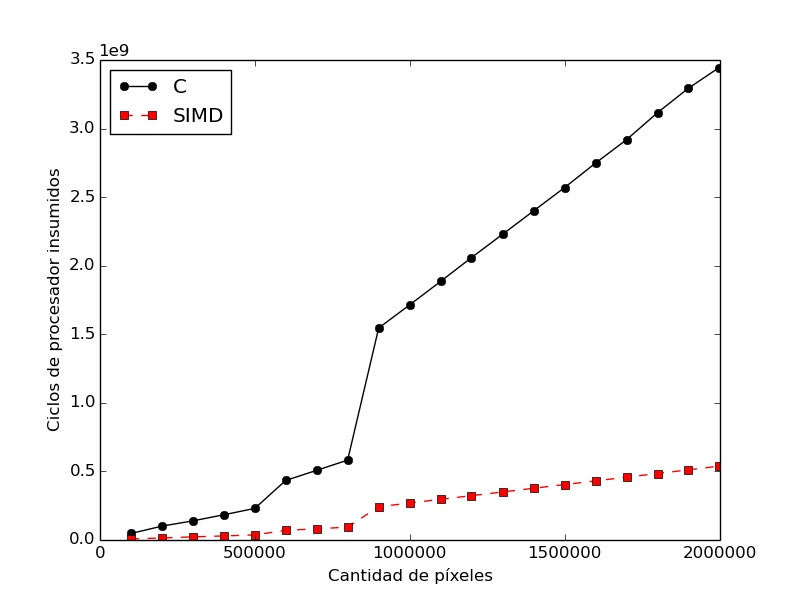
\includegraphics[scale=0.5]{graph1.jpg}
	\end{center}		
	\caption{Tiempo de ejecución del algoritmo de trazado de rayos}
	\label{fig2}
\end{figure}

Ahora vemos los resultados exactos, para poder calcular exactamente la mejora de performance:\\

\begin{center}
\begin{tabular}[H]{|c|c|c|c|}\hline
$i_w \times i_h$ & \textbf{C} & \textbf{SIMD} & \textbf{C/SIMD} \\\hline
99645 & 47412965.4 & 7458009.6 & 6.35\\
199692 & 101101387.08 & 14760852.94 & 6.84\\
299568 & 139660581.06 & 22901589.62 & 6.09\\
399310 & 183821009.3 & 29576126.24 & 6.21\\
499392 & 230551223.58 & 37123983.44 & 6.21\\
598980 & 434228563.54 & 70736674.38 & 6.13\\
699384 & 508383989.28 & 81353151.38 & 6.24\\
798768 & 582486590.68 & 94119090.62 & 6.18\\
898995 & 1545718116.28 & 242396510.46 & 6.37\\
999364 & 1715182797.38 & 269795128.46 & 6.35\\
1099588 & 1887044517.02 & 296972078.78 & 6.35\\
1198272 & 2059100630.34 & 323324739.4 & 6.36\\
1298892 & 2229584118.58 & 350339094.04 & 6.36\\
1398784 & 2399859498.14 & 377197091.18 & 6.36\\	
1498840 & 2569943753.52 & 404182225.46 & 6.35\\
1598700 & 2748590124.28 & 430763849.88 & 6.38\\
1699145 & 2919986197.18 & 458490048.64 & 6.36\\
1798389 & 3115715808.92 & 484714280.96 & 6.42\\
1898063 & 3294098954.12 & 511512759.16 & 6.43\\
1997568 & 3445162034.08 & 538688063.42 & 6.39\\\hline

\end{tabular}
\end{center}

Como vemos en la figura 2, la implementación SIMD es más de 6 veces más rápida que la implementación C. También vemos que la diferencia de performance se mantiene constante cambiando la resolución. Esperabamos que el aumento de performance fuera de $3x$ aproximadamente, ya que en la mayoría de las operaciones, se manejan tres variables al mismo tiempo en vez de una. Entonces, consideramos que esa mejora de la performance mayor se debe al cambio de las funciones a macros y a que, programando a bajo nivel, se puede programar más eficientemente que en C al poner todas las variables en registros y eliminando las que no se necesitan.
También, notamos dos saltos en tiempo de ejecución considerables, a partir de $5 \times 10^6$ píxeles y a partir de $9 \times 10^6$. Consideramos que esto es porque a partir de esos números los datos dejan de caber en la memoria caché del procesador, entonces el programa tarda más tiempo en recuperar los datos de memoria.

\end{document}